\chapter{Aufgabenanalyse}\label{ch:aufgabenanalyse}


\section{Interpretation der Aufgabe}\label{sec:interpretation-der-aufgabe}
Zur Auswertung von Signalen eines optischen Autokorrelators soll ein Programm entwickelt werden.
Der Autokorrelator liefert fortlaufend Daten, die vom Programm eingelesen, verarbeitet und ausgegeben werden.
Weil diese Schritte für unterschiedliche Datensätze unterschiedliche Laufzeiten haben, sollen sie in voneinander unabhängigen Threads laufen.

Die einzelnen Datensätze werden zum Test in zehn unterschiedlichen Textdateien zur Verfügung gestellt.
Diese sind durchnummeriert von null bis neun und haben die folgende Namenskonvention:
\begin{center}
    <nummer>.txt
\end{center}
Ein Datensatz enthält jeweils $N$ Messdaten, die aus zwei positiven Ganzzahlen bestehen.
Die erste Zahl steht dabei für die Intensität des Messsignals und wird im Folgenden als y-Wert interpretiert.
Die zweite Zahl bezeichnet die Spiegelposition und wird als \~x-Wert interpretiert.
Der Spiegel ist eine Komponente des Autokorrelators, die vor und zurück bewegt werden kann, um das Output-Signal zu manipulieren.

Der einlesende Thread soll die zehn Textdateien in chronologischer Reihenfolge einlesen und in eine geeignete Datenstruktur überführen.
Wenn die zehnte Datei fertig bearbeitet wurde, soll wieder bei der ersten begonnen werden.
Dieses Verhalten wird fortgesetzt, bis ein Signal zum Programmabbruch empfangen wird.
Es soll hier das Verhalten im produktiven Betrieb simuliert werden, in dem nicht nur zehn Datensätze bearbeitet werden, sondern fortlaufend neue Datensätze vom Autokorrelator produziert werden.
Der Einlese-Thread stellt jeden Datensatz für 0,05 Sekunden zur Abholung über eine Schnittstelle zur Verfügung.

Der Verarbeitungs-Thread holt sich über diese Schnittstelle Datensätze, führt diverse Transformationen und Berechnungen durch und sendet die Ergebnisse an den Ausgabe-Thread.
Es werden nur Datensätze verarbeitet, die die Verarbeitung vorher noch nicht durchlaufen haben.
Auch die Verarbeitung läuft, bis ein Signal zum Programmabbruch empfangen wird.

Gleiches gilt für den Ausgabe-Thread.
Dieser bietet eine Schnittstelle, über die verarbeitete Datensätze angenommen werden.
Die Ergebnisse werden wieder in eine Textdatei geschrieben.
Wenn die Ausgabe eines Datensatzes erfolgreich war, wird das an zentraler Stelle vermerkt.
So kann erkannt werden, wenn alle Eingabedateien erfolgreich verarbeitet und ausgegeben wurden.
Dann ist das Kriterium zum Programmende erreicht und alle Threads können beendet werden.

\section{Eingabeformat}\label{sec:eingabe-format}
Wie bereits beschrieben, liegen die Datensätze in Textdateien.
In diesen Dateien sind die einzelnen Messpunkte, bestehend aus \~x- und y-Wert, zeilenweise zu finden.
An erster Stelle steht der y-Wert.
Getrennt durch einen Tabulator folgt der \~x-Wert.
Zeilen die mit einem \#-Zeichen beginnen sind Kommentare und können ignoriert werden.
\begin{figure}[htb]
    \centering
    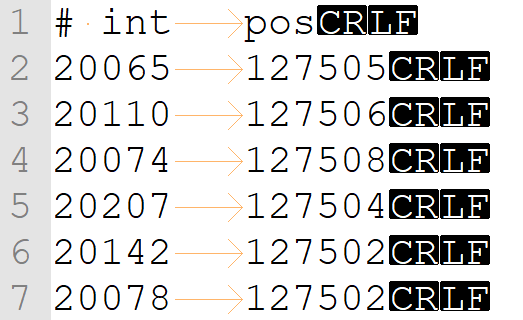
\includegraphics[width=0.5\linewidth]{images/eingabeDat_bsp}
    \caption{
        Beispielausschnitt einer Eingabedatei.
    }
    \label{fig:eingabe_dat_beispiel}
\end{figure}


\section{Ausgabeformat}\label{sec:ausgabeformat}
Nach erfolgreicher Verarbeitung werden die Ergebnisse wieder in eine Textdatei geschrieben.
Diese Dateien haben den Namen der zugehörigen Eingabedatei mit dem zusätzlichen Präfix \enquote{out}.
Die Eingabedatei \enquote{1.txt} hat dann z.B. \enquote{out1.txt}.

In die erste Zeile werden die Informationen zur berechneten Pulsbreite (siehe Abschnitt~\ref{subsec:pulsbreite}) geschrieben.
Dabei soll das folgende Format verwendet werden:
\begin{center}
    \# FWHM = <Pulsbreite:float>, <Links-Index:int>, <Rechts-Index:int>
\end{center}
In den folgenden Zeilen sollen wieder zeilenweise die verarbeiteten Messpunkte stehen.
Pro Zeile werden, jeweils getrennt durch einen Tabulator, erwartet:
\begin{itemize}[noitemsep]
    \item Der umgeformte und geglättete \~x-Wert (siehe Abschnitt~\ref{subsec:glaettung}).
    \item Der skalierte y-Wert (siehe Abschnitt~\ref{subsec:umrechnung-und-normierung}).
    \item Der Wert der oberen Einhüllenden (siehe Abschnitt~\ref{subsec:ober-einh}) an der passenden Stelle.
\end{itemize}

\begin{figure}[htb]
    \centering
    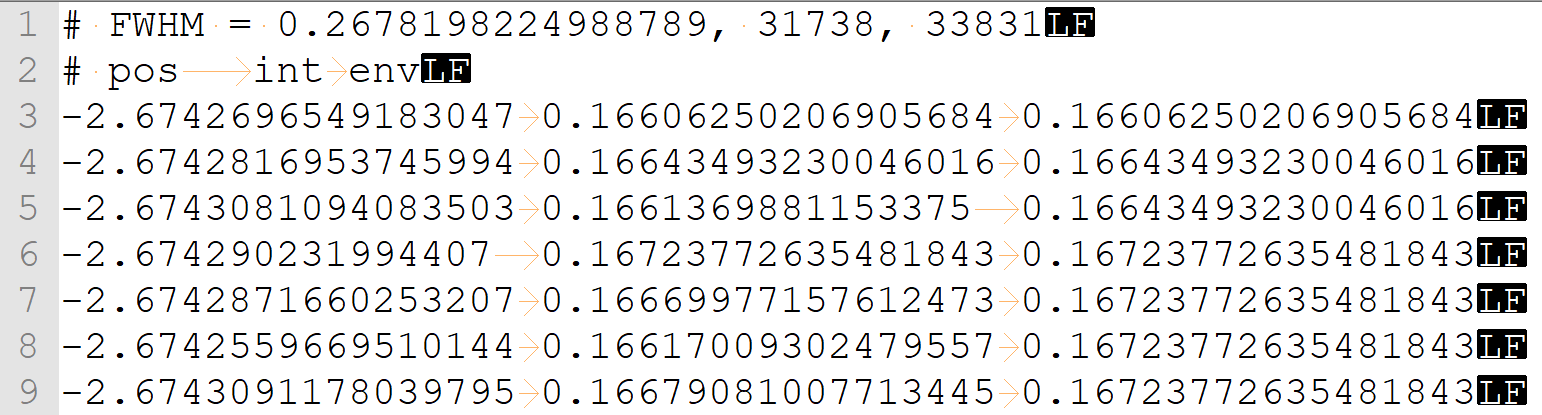
\includegraphics[width=\linewidth]{images/ausgabeDat_bsp}
    \caption{
        Beispielausschnitt einer Ausgabedatei.
    }
    \label{fig:ausgabe_dat_beispiel}
\end{figure}

\section{Fehlerarten}\label{sec:fehlerarten}
Beim ausführen des Programms kann es zu unterschiedlichen Fehlern kommen.
Diese werden im Folgenden beschrieben.

\subsection{Technische Fehler}\label{subsec:technische-fehler}
Das Programm geht davon aus, dass die Anzahl der Testdateien mit dem angegebenen Wert übereinstimmt und dass die Dateien die oben genannte Namenskonvention einhalten.
Ist das nicht der Fall, werden Fehler geworfen.

Es kann auch sein, dass eine Datei beim Zugriff blockiert ist (z.B. durch ein anderes Programm oder wegen fehlenden Berechtigungen).
Dies würde ebenso zu einer Fehlersituation führen.

Auch bei der Ausgabe kann es beim Schreiben der Dateien aus selbigen Gründen zu technischen Fehler kommen.

\subsection{Syntaktische Fehler}\label{subsec:syntaktische-fehler}
Syntaktische Fehler treten auf, wenn die Eingabedateien nicht im richtigen Format vorliegen (Siehe Abschnitt~\ref{sec:eingabe-format}).
Z.B. wenn an Stelle des Tabulators ein anderes Trennzeichen verwendet wird oder mehr als zwei Einträge in einer Zeile zu finden sind.

\subsection{Semantische Fehler}\label{subsec:semantische-fehler}
Auch semantische Fehler müssen bei der Eingabe überprüft werden.
Es sind in den Eingabedateien nur positive Ganzzahlen als \~x- und y-Werte erlaubt.
Außerdem sollten mindestens 500 gültige Einträge pro Datei vorhanden sein.
Sonst kommt es beim Glätten der \~x-Werte nach der Berechnung $n = \lfloor 0.002 \cdot N \rfloor - 1$ zu Problemen.
Ist $N$ hier kleiner als 500, dann wird $n$ negative und eignet sich nicht als Intervallgröße.

\section{Fehlerbehandlung}\label{sec:fehlerbehandlung}
Die oben spezifizierten Fehler benötigen alle eine sinnvolle Fehlerbehandlung.
Diese wird nun festgelegt.

\subsection{Technische Fehler}\label{subsec:technische-fehler-behandlung}
Wenn eine Datei sich nicht zum Lesen oder Schreiben öffnen lässt, sollte eine entsprechende Meldung auf der Konsole ausgegeben werden.
Zudem sollte diese Datei in der Programmsteuerung als bearbeitet markiert werden, bzw. der Zähler der bearbeiteten Dateien hochgezähl werden.
Ansonsten würde das Programm endlos weiterlaufen.

\subsection{Syntaktische und Semantische Fehler}\label{subsec:syntaktische-semant-fehler-behandlung}
Fehlerhafte Zeilen in den Eingabedateien werden ebenfalls auf der Konsole gemeldet und für die Verarbeitung ignoriert.
Hat eine Datei in mehr als 50\% der Zeilen syntaktische oder semantische Fehler, wird sie nicht weiterverarbeitet.
Selbiges gilt, wenn weniger als 500 fehlerfreie Einträge vorhanden sind.



%\subsection{Sonderfälle}\label{subsec:sonderfaelle}
